\section{Figures}

\begin{figure}[h]
  \centering
  \includegraphics[width=0.95\textwidth]{LEU_ILE_HIS}
  \caption{\FigOneCaption}
    \label{fig:outcontour}
\end{figure}



\begin{figure}[h]
  \centering
  \includegraphics[width=0.95\textwidth]{contour_compare}
  \caption{\FigTwoCaption}
    \label{fig:contour_compare}
\end{figure}



\begin{figure}[h]
  \centering
  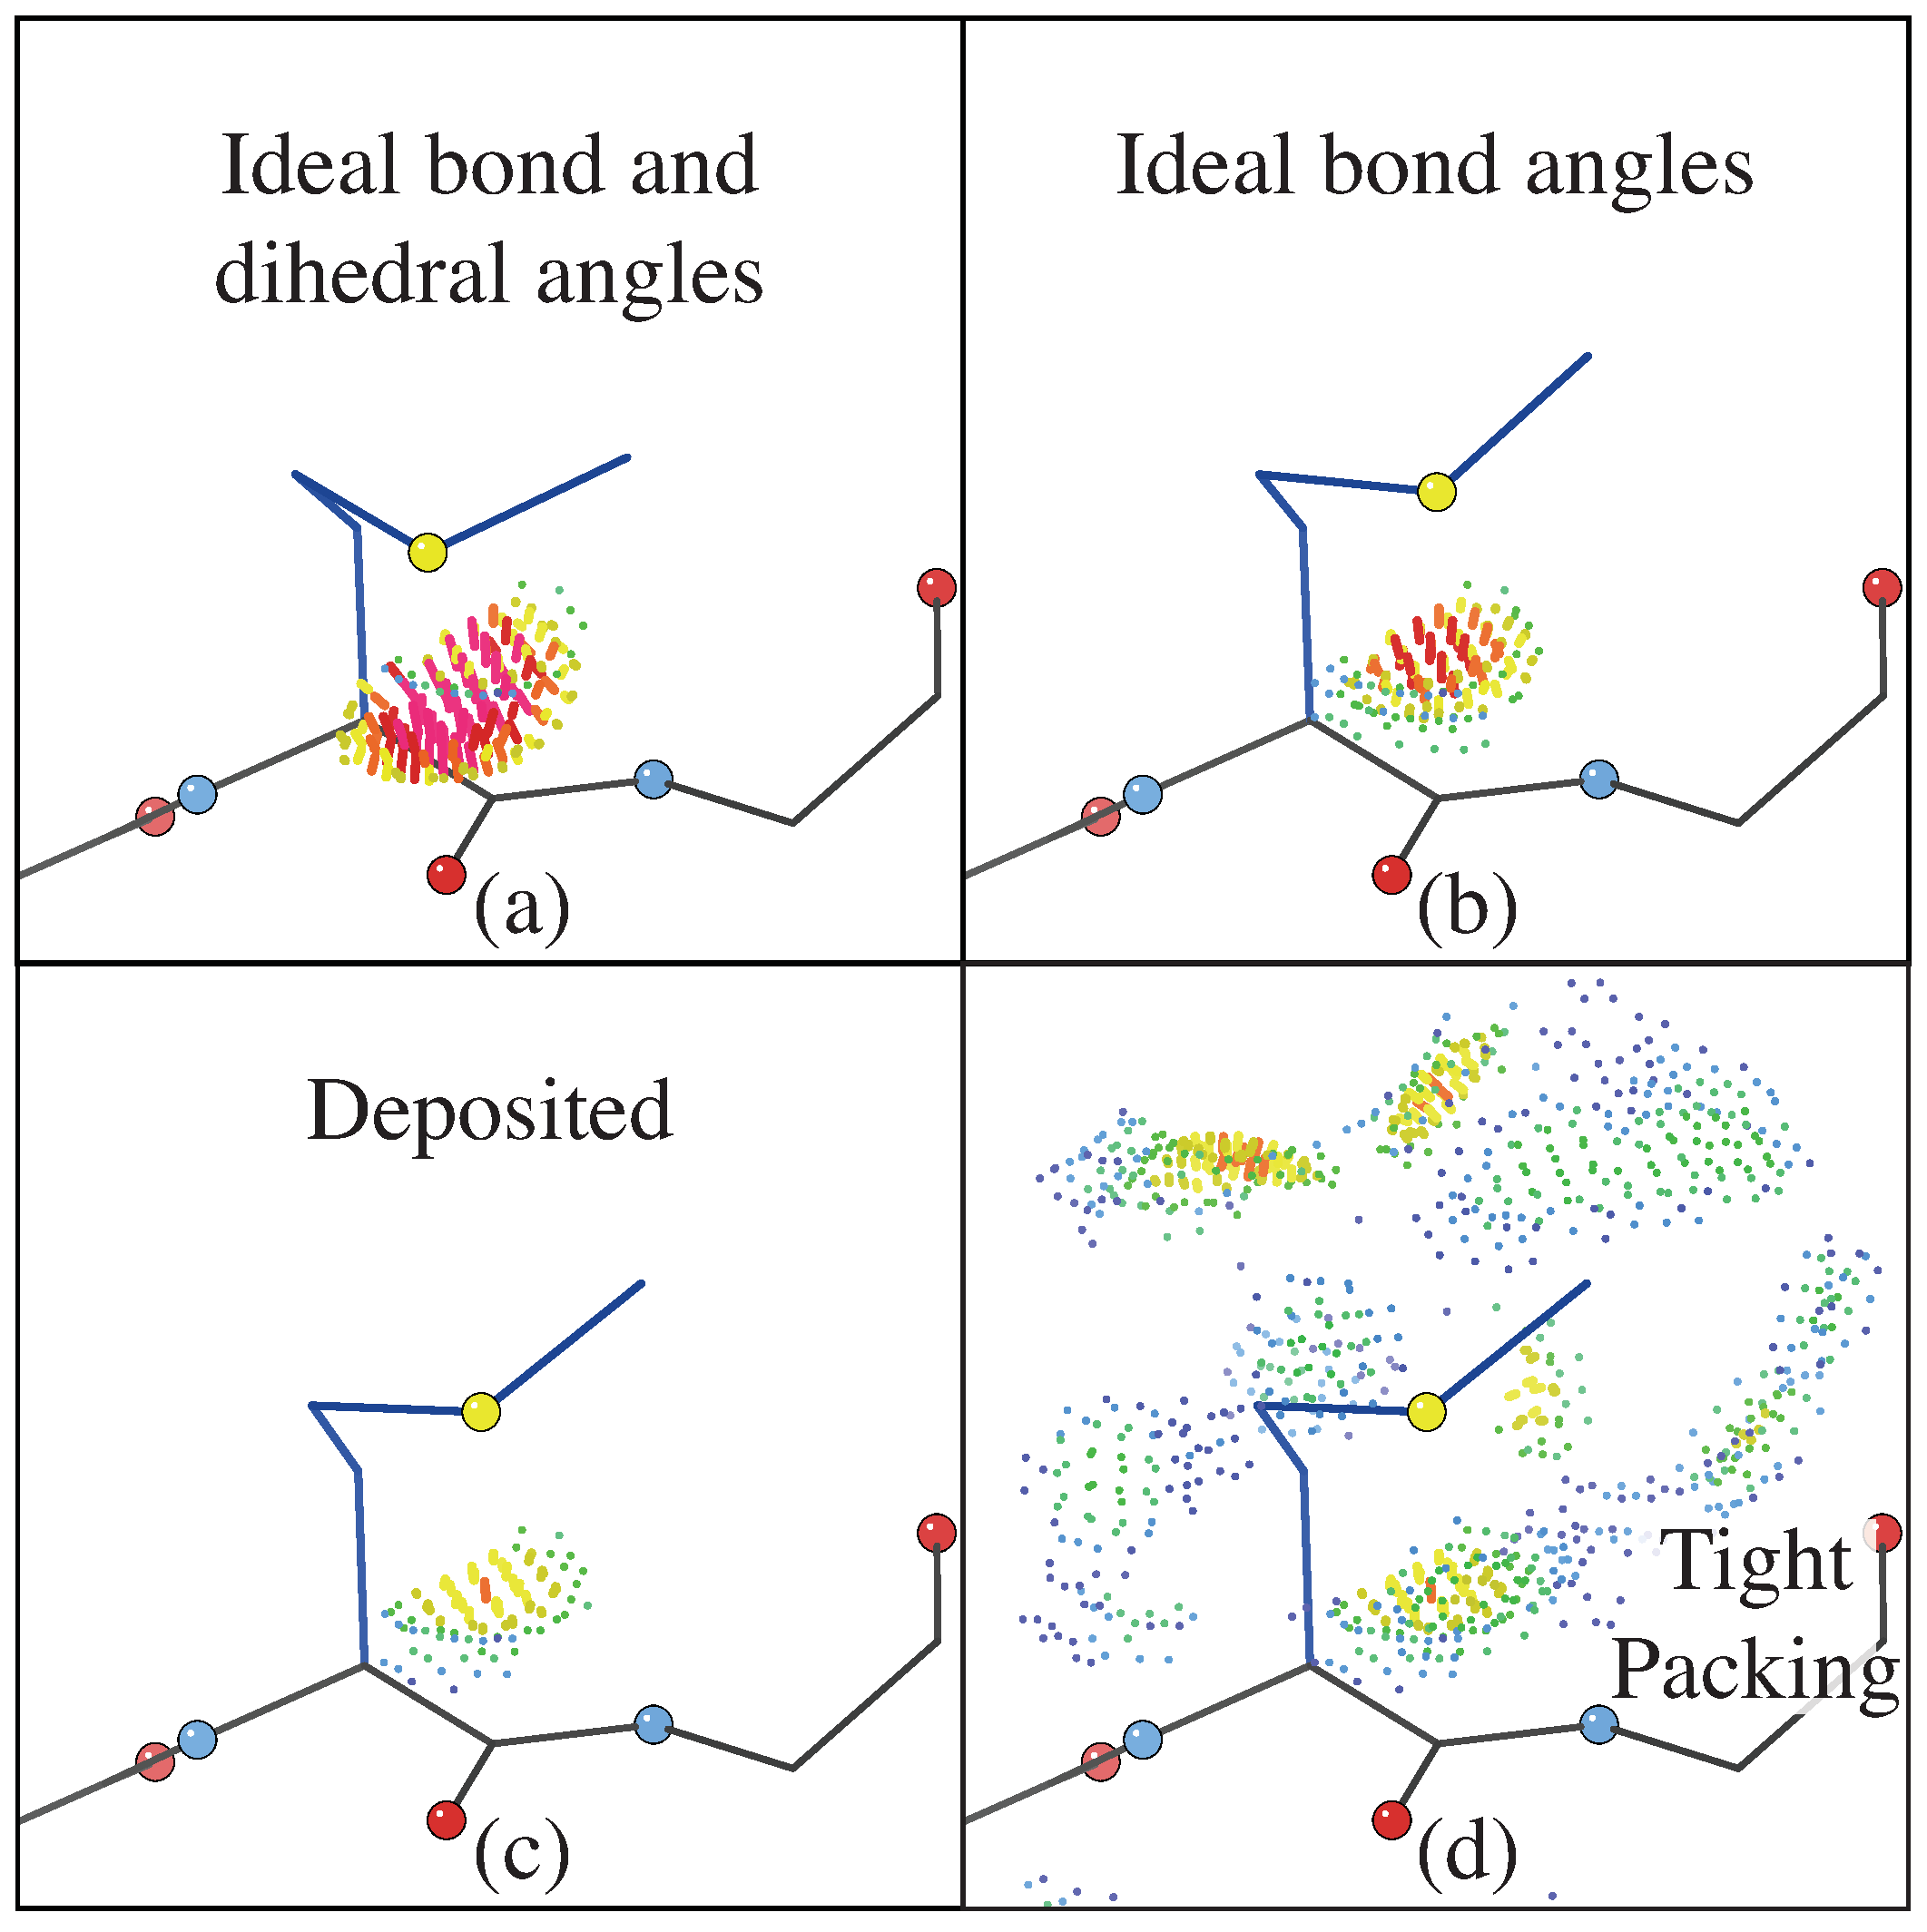
\includegraphics[width=0.5\textwidth]{MetPPP}
  \caption{\FigThreeCaption}
    \label{fig:2bmo}
\end{figure}



\begin{figure}[h]
  \centering
  \includegraphics[width=0.75\textwidth]{Glu_pm20_mp0}
\caption{\FigFourCaption}
\label{fig:Glupm20_mp0}
\vspace{-10pt}
\end{figure}


\begin{figure}[h]
  \centering
  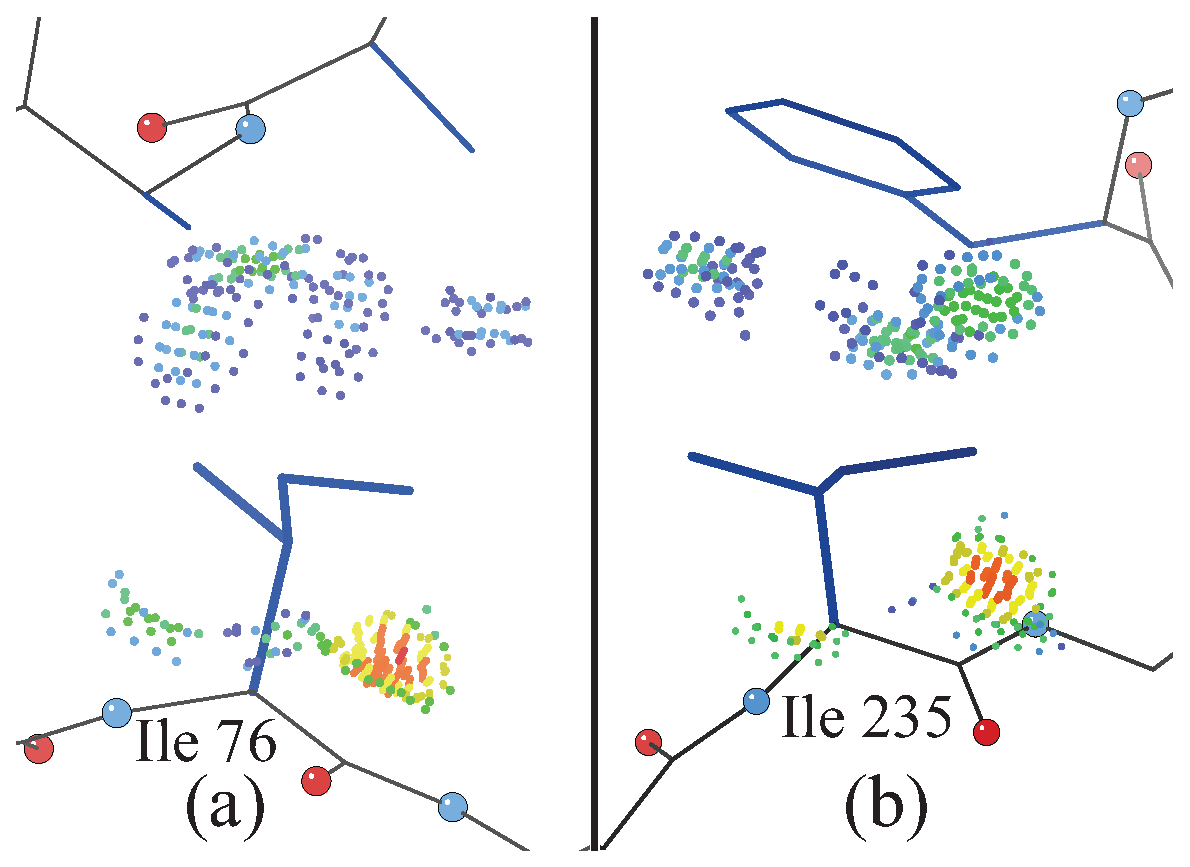
\includegraphics[width=0.5\textwidth]{IlePP}
\caption{\FigFiveCaption}
\label{fig:Ilepp}
\vspace{-10pt}
\end{figure}


\begin{figure}[h]
  \centering
  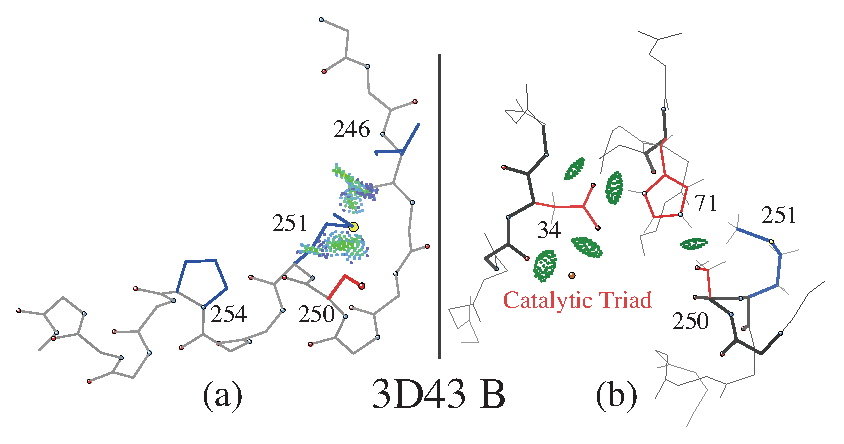
\includegraphics[width=0.95\textwidth]{Metmpm}
\caption{\FigSixCaption}
\label{fig:METmpm_3d43}
\vspace{-10pt}
\end{figure}


\begin{figure}[h]
  \centering
  \includegraphics[width=0.85\textwidth]{AspAsn_contours}
\caption{\FigSevenCaption}
\label{fig:AspAsn}
\vspace{-10pt}
\end{figure}



\begin{figure}[h]
  \centering
  \includegraphics[width=0.65\textwidth]{ASN_outliers}
\caption{\FigEightCaption}
\label{fig:AsnOutliers}
\vspace{-10pt}
\end{figure}
